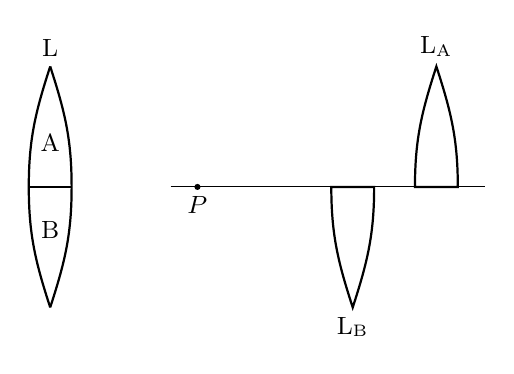
\begin{tikzpicture}[scale=0.85,font=\small]
  % Left: original lens L split into A and B
  \begin{scope}[shift={(0,0)}]
    \draw[thick] (0, 1.8) to[out=-108,in=90] (-0.32, 0) to[out=-90,in=108] (0, -1.8);
    \draw[thick] (0, 1.8) to[out=-72,in=90] (0.32, 0) to[out=-90,in=72] (0, -1.8);
    \draw[thick] (-0.32, 0) -- (0.32, 0);
    \node[above] at (0, 1.8) {L};
    \node at (0, 0.65) {A};
    \node at (0, -0.65) {B};
  \end{scope}

  % Right: Meslin split lens with P, L_B, L_A
  \begin{scope}[shift={(4.4,0)}]
    % Optical axis
    \draw[thin] (-2.6, 0) -- (2.1, 0);
    % Point source P
    \fill (-2.2, 0) circle (1.3pt) node[below] {$P$};
    % Lower half L_B
    \draw[thick] (-0.2, 0) to[out=-90,in=108] (0.12, -1.8) to[out=72,in=-90] (0.44, 0) -- cycle;
    \node[below] at (0.12, -1.8) {$\mathrm{L_B}$};
    % Upper half L_A shifted right
    \draw[thick] (1.05, 0) to[out=90,in=-108] (1.37, 1.8) to[out=-72,in=90] (1.69, 0) -- cycle;
    \node[above] at (1.37, 1.8) {$\mathrm{L_A}$};
  \end{scope}
\end{tikzpicture}
